\documentclass[letterpaper,11pt]{article}
\oddsidemargin -1.0cm \textwidth 17.5cm

\usepackage[utf8]{inputenc}
\usepackage[activeacute,spanish, es-lcroman]{babel}
\decimalpoint
\usepackage{amsfonts,setspace}
\usepackage{amsmath}
\usepackage{amssymb, amsmath, amsthm}
\usepackage{comment}
\usepackage{float}
\usepackage{amssymb}
\usepackage{dsfont}
\usepackage{anysize}
\usepackage{multicol}
\usepackage{enumerate}
\usepackage{graphicx}
\usepackage[left=1.5cm,top=2cm,right=1.5cm, bottom=1.7cm]{geometry}
\setlength\headheight{1.5em} 
\usepackage{fancyhdr}
\usepackage{multicol}
\usepackage{hyperref}
\usepackage{wrapfig}
\usepackage{subcaption}
\usepackage{siunitx}
\usepackage{cancel}
\usepackage{mdwlist}
\usepackage{svg}
\pagestyle{fancy}
\fancyhf{}
\renewcommand{\labelenumi}{\normalsize\bfseries P\arabic{enumi}.}
\renewcommand{\labelenumii}{\normalsize\bfseries (\alph{enumii})}
\renewcommand{\labelenumiii}{\normalsize\bfseries \roman{enumiii})}


\begin{document}

\fancyhead[L]{\itshape{Facultad de Ciencias F\'isicas y Matem\'aticas}}
\fancyhead[R]{\itshape{Universidad de Chile}}

\begin{minipage}{11.5cm}
    \begin{flushleft}
        \hspace*{-0.6cm}\textbf{FI1000-1 Introducción a la Física Clásica}\\
        \hspace*{-0.6cm}\textbf{Profesora:} Jocelyn Dunstan\\
        \hspace*{-0.6cm}\textbf{Auxiliar:} Alejandro Silva\\
        \hspace*{-0.6cm}\textbf{Ayudantes:} Macarena Muñoz \& Catalina Vargas\\
    \end{flushleft}
\end{minipage}

\begin{picture}(2,3)
    \svgpath{../}  % descomentar si se agrega a carpeta "auxiliares"/"ejercicios"
    \put(366, 10){\includesvg[scale=0.31]{img/dfi.svg}}
\end{picture}

\begin{center}
	\LARGE\textbf{Auxiliar \#6}\\
	\Large{Roce y Ley de Hooke}
\end{center}

\vspace{-1cm}
\begin{enumerate}\setlength{\itemsep}{0.4cm}

\rfoot[]{pág. \thepage}

\item[]

\item La última atracción de Fantasilandia es un tambor de radio $R$ que gira sobre su eje suficientemente rápido de modo que una persona parada en su interior es mantenida erguida contra las paredes cuando la parte inferior del tambor se deja caer. Si el coeficiente de roce estático y cinético son $\mu_e$ y $\mu_c$ respectivamente, determine la rapidez angular $\omega$ mínima del tambor que evita que las personas se caigan.

\item Un bloque de masa $m$ se encuentra unido a un resorte de constante elástica $k$ y largo natural nulo, cuyo extremo está a una altura $H$ de una cinta sobre la cual se apoya el bloque. Esta cinta posee un coeficiente de roce estático $\mu_e$ y cinético $\mu_c$, y se mueve con rapidez $v_0$ hacia la derecha. Determine a qué ángulo $\beta$ el bloque comienza a deslizarse. 

\begin{figure}[H]
    \centering
    \begin{subfigure}[t]{0.45\textwidth}
        \centering
        \svgpath{../img/aux6}
        \includesvg[width=0.5\linewidth]{tambor.svg}
        \caption{P1}
    \end{subfigure}
    \begin{subfigure}[t]{0.45\textwidth}
        \centering
        \svgpath{../img/aux6}
        \includesvg[width=0.8\linewidth]{riel.svg} 
        \caption{P2}
    \end{subfigure}
\end{figure}

\item Un aro de radio $R$ dispuesto en forma vertical se mueve horizontalmente como se indica en la figura. En el punto $O$ se fija el extremo de un resorte de constante elástica $k$ y de largo natural $\ell_0 = \pi R /2$. En el otro extremo del resorte se adhiere una argolla de masa $m$. El resorte envuelve el aro de modo que su forma es siempre la de un arco de círculo de radio $R$. A consecuencia del movimiento del aro, el resorte mantiene una elongación constante caracterizada por un arco de ángulo $\theta$ con respecto al eje del aro. Determine la aceleración del aro.

\item\textbf{[Propuesto]} De las dos siguientes configuraciones, ¿cuál de ellas produce la mayor elongación del extremo inferior?

\begin{figure}[H]
    \centering
    \begin{subfigure}[t]{0.45\textwidth}
        \centering
        \svgpath{../img/aux6}
        \includesvg[width=0.8\linewidth]{aro.svg}     
        \caption{P3}
    \end{subfigure}
    \begin{subfigure}[t]{0.45\textwidth}
        \centering
        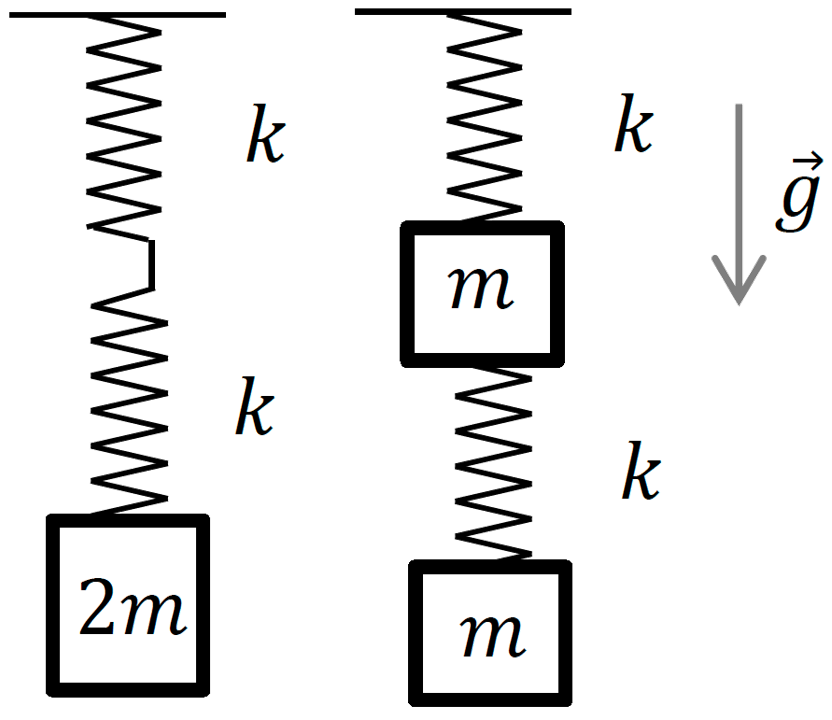
\includegraphics[scale=0.2]{2021-2/img/aux6/resortes.png}
        \caption{P4}
    \end{subfigure}
\end{figure}

% Para imágenes vectoriales -> el texto tiene que estar en LaTeX
% \begin{figure}[htbp]
%   \centering
%   \svgpath{../Imagenes/ejercicios}  -> .. irse pa'trás 
%   \includesvg{ej5.svg}
% \end{figure}

\end{enumerate}
\end{document}
